\section{Diseño Básico del Husillo}
Para el básico del sistema de corte motor-husillo se toma como guía los catálogos de herramientas de corte  \cite{catalogue:CatalogoC006s} y \cite{catalogue:Blue_Master} , para asi obtener los parámetros corte y variables a considerar para el cálculo de potencia de corte ($P_c$). 

\subsection{Parámetros de corte recomendados para fresas HSS-Co8}

En el dimensionamiento del motor-husillo se utilizaron parámetros de corte recomendados por el fabrícate de fresas \cite{catalogue:Blue_Master} donde especifica las velocidades de corte ($V_C$) y velocidades de avance($V_f$) dependiendo del material del que está hecha la pieza de trabajo y las características de la herramienta de corte fresa. En este mismo catalogo también recomiendo ancho de corte($e_p$) y profundidad de corte ($a_p$), los cuales depende del diámetro de la herramienta de corte y el tipo de operación.. Los diámetros con lo que se quiere trabajar en las operaciones de fresado esta entre 2 a 18 mm y los materiales de las piezas a trabajar serán aluminio y acero blando. Los parámetros se presentaron en la tabla \ref{table:Parametro_de_corte}.\\


% Please add the following required packages to your document preamble:
% \usepackage{multirow}
% \usepackage[table,xcdraw]{xcolor}
% If you use beamer only pass "xcolor=table" option, i.e. \documentclass[xcolor=table]{beamer}
\begin{longtable}{|c|c|c|c|c|c|c|c|}\hline
\rowcolor[HTML]{EFEFEF} 
\multicolumn{3}{|c|}{\cellcolor[HTML]{EFEFEF}} & \multicolumn{5}{c|}{\cellcolor[HTML]{EFEFEF}Diametro (mm)} \\ \cline{4-8} 
\rowcolor[HTML]{EFEFEF} 
\multicolumn{3}{|c|}{\multirow{-2}{*}{\cellcolor[HTML]{EFEFEF}}}                                                                                                                                                                                    & 2   & 4  & 8  & 10& 18\\ \hline
\rowcolor[HTML]{EFEFEF} 
\cellcolor[HTML]{EFEFEF}  & \begin{tabular}[c]{@{}c@{}}Velocidad de \\ corte (m / min)\end{tabular}  & \cellcolor[HTML]{EFEFEF}  & \multicolumn{5}{c|}{\cellcolor[HTML]{EFEFEF}Velocidad angular(RPM)} \\ \cline{2-2} \cline{4-8} 
\rowcolor[HTML]{EFEFEF} 
\cellcolor[HTML]{EFEFEF}                                                                                                                                       & 39                                                                                        & \multirow{-2}{*}{\cellcolor[HTML]{EFEFEF}N ° de filos} & 6207         & 3104         & 1552        & 1241        & 690       \\ \cline{2-8} 
\cellcolor[HTML]{EFEFEF}                                                                                                                                       &                                                                                           & 2                                                      & 50           & 56           & 84          & 82          & 80        \\ \cline{3-8} 
\cellcolor[HTML]{EFEFEF}                                                                                                                                       &                                                                                           & 3                                                      & 75           & 84           & 126         & 123         & 120       \\ \cline{3-8} 
\multirow{-5}{*}{\cellcolor[HTML]{EFEFEF}\begin{tabular}[c]{@{}c@{}}Acero blando \\ \\ Resistencia a la tracción \\  70 Kg / mm \textasciicircum 2\end{tabular}} & \multirow{-3}{*}{\begin{tabular}[c]{@{}c@{}}Velocidad de \\ avance (mm/min)\end{tabular}} & 4                                                      & 100          & 112          & 168         & 164         & 160       \\ \hline
\rowcolor[HTML]{EFEFEF} 
\cellcolor[HTML]{EFEFEF}                                                                                                                                       & \begin{tabular}[c]{@{}c@{}}Velocidad de \\ corte (m / min)\end{tabular}                   & \cellcolor[HTML]{EFEFEF}                               & \multicolumn{5}{c|}{\cellcolor[HTML]{EFEFEF}Velocidad angular(RPM)} \\ \cline{2-2} \cline{4-8} 
\rowcolor[HTML]{EFEFEF} 
\cellcolor[HTML]{EFEFEF}                                                                                                                                       & 230                                                                                       & \multirow{-2}{*}{\cellcolor[HTML]{EFEFEF}N ° de filos} & 36606        & 18303        & 9152        & 7321        & 4067      \\ \cline{2-8} 
\cellcolor[HTML]{EFEFEF}                                                                                                                                       &                                                                                           & 2                                                      & 293          & 329          & 494         & 400         & 230       \\ \cline{3-8} 
\cellcolor[HTML]{EFEFEF}                                                                                                                                       &                                                                                           & 3                                                      & 440          & 494          & 741         & 600         & 345       \\ \cline{3-8} 
\multirow{-5}{*}{\cellcolor[HTML]{EFEFEF}Aluminio}                                                                                                             & \multirow{-3}{*}{\begin{tabular}[c]{@{}c@{}}Velocidad de \\ avance (mm/min)\end{tabular}} & 4                                                      & 586          & 658          & 988         & 800         & 460       \\ \hline
\caption{Parametros de corte para el Acero blando y aluminio}{Fuente:\citep{catalogue:Blue_Master}}
\label{table:Parametro_de_corte}
\end{longtable}

En la Figura \ref{fig:Profun} se presenta las profundidades recomendadas para tres distintas operaciones.  

\begin{figure}[hbt]
    \centering
    \begin{subfigure}{0.3\textwidth}
        \centering
        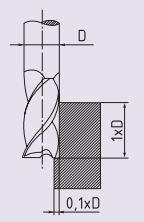
\includegraphics[width=0.9\linewidth]{Cap4_DisenoBasico/Figura/Fresado_Lateral.PNG}
        \caption{Fresado Lateral}
        \label{fig:Fresado_Lateral}
    \end{subfigure} 
    \centering
    \begin{subfigure}{0.3\textwidth}
        \centering
        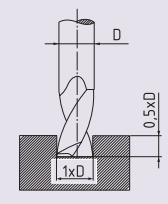
\includegraphics[width=0.9\linewidth]{Cap4_DisenoBasico/Figura/Ranurado.PNG}
        \caption{Vaciado}
        \label{fig:VAciado}
    \end{subfigure} 
    \centering
    \begin{subfigure}{0.3\textwidth}
        \centering
        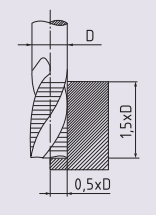
\includegraphics[width=0.9\linewidth]{Cap4_DisenoBasico/Figura/Basto.PNG}
        \caption{Basto}
        \label{fig:Basto}
    \end{subfigure} 
    \caption{Profucidad y ancho de corte recomendada del fresado}{Fuente: \citep{catalogue:Blue_Master}}
    \label{fig:Profun}
\end{figure}

Para preservar la vida útil de herramienta de corte y tener un menor consumo de potencia se plantea que para el aluminio en el fresado Basto la profundidad corte ($a_p$) a partir del diámetro de 8 mm en adelante será de 10 $mm$ y para el fresado ranurado o vaciado la profundidad es $0.3$ el diametro de la fresa. De igual forma para el acero blando se toma tambien una progundidad de corte similar a la de fresado basto pero el ancho de corte será $0.25$ el diametro de la herramienta, y en el ranurado la profundidad de corte será $0.2$ el diametro de la herramineta de fresado. En la tabla \ref{table:Profundidad_aluminio} y la tabla \ref{table:Profundidad_acero} se presentará el ancho y profundidad de corte para los tipos de fresado .

Con los parámetros ya obtenidos, se procede a usar la expresión encontrada en catálogo de \cite{catalogue:CatalogoC006s} donde,  relacionan los parámetros de corte con un término llamado presión especifica de corte que esta tabulada con respecto al avance por diente. La ecuacion \ref{Eq:P_c} es la expresión para el calculo de la potencia de corte.

% Please add the following required packages to your document preamble:
% \usepackage[table,xcdraw]{xcolor}
% If you use beamer only pass "xcolor=table" option, i.e. \documentclass[xcolor=table]{beamer}

\begin{longtable}{|>{\columncolor[HTML]{EFEFEF}}c |c|c|c|c|c|c|}
\hline
\multicolumn{2}{|c|}{\cellcolor[HTML]{EFEFEF}Diametro ($mm$)}                  & \multicolumn{1}{l|}{\cellcolor[HTML]{EFEFEF}2} & \multicolumn{1}{l|}{\cellcolor[HTML]{EFEFEF}4} & \multicolumn{1}{l|}{\cellcolor[HTML]{EFEFEF}8} & \multicolumn{1}{l|}{\cellcolor[HTML]{EFEFEF}10} & \multicolumn{1}{l|}{\cellcolor[HTML]{EFEFEF}18} \\ \hline
\multicolumn{7}{|c|}{\cellcolor[HTML]{EFEFEF}Fresado Lateral}   \\ \hline
\begin{tabular}[c]{@{}c@{}}Profundidad\\   de corte (mm)\end{tabular} & ap & 2& 4 & 8& 10& 18\\ \hline
\begin{tabular}[c]{@{}c@{}}Ancho de\\   corte (mm)\end{tabular}       & ep & 0,2& 0,4 & 0,8& 1& 1,8\\ \hline
\multicolumn{7}{|c|}{\cellcolor[HTML]{EFEFEF}Vaciado} \\ \hline
\begin{tabular}[c]{@{}c@{}}Profundidad\\   de corte(mm)\end{tabular}  & ap & 0,6 & 1,2 & 2,4 & 3 & 5,4\\ \hline
\begin{tabular}[c]{@{}c@{}}Ancho de\\   corte(mm)\end{tabular}        & ep & 2 & 4 & 8 & 10 & 18 \\ \hline
\multicolumn{7}{|c|}{\cellcolor[HTML]{EFEFEF}Basto}\\ \hline
\begin{tabular}[c]{@{}c@{}}Profundidad\\   de corte(mm)\end{tabular}  & ap & 3& 6& 10 & 10 & 10\\ \hline
\begin{tabular}[c]{@{}c@{}}Ancho de\\   corte(mm)\end{tabular} & ep & 1  & 2 & 4 & 5 & 9  \\ \hline

\caption{Profundidad y ancho de corte para aluminio}{Fuente:\cite{catalogue:Blue_Master}}
\label{table:Profundidad_aluminio}
\end{longtable}



% Please add the following required packages to your document preamble:
% \usepackage[table,xcdraw]{xcolor}
% If you use beamer only pass "xcolor=table" option, i.e. \documentclass[xcolor=table]{beamer}

\begin{longtable}{|>{\columncolor[HTML]{EFEFEF}}c |c|c|c|c|c|c|}
\hline
\hline
\multicolumn{2}{|c|}{\cellcolor[HTML]{EFEFEF}Diametro ($mm$)} & \multicolumn{1}{l|}{\cellcolor[HTML]{EFEFEF}2} & \multicolumn{1}{l|}{\cellcolor[HTML]{EFEFEF}4} & \multicolumn{1}{l|}{\cellcolor[HTML]{EFEFEF}8} & \multicolumn{1}{l|}{\cellcolor[HTML]{EFEFEF}10} & \multicolumn{1}{l|}{\cellcolor[HTML]{EFEFEF}18} \\ \hline
\multicolumn{7}{|c|}{\cellcolor[HTML]{EFEFEF}Fresado Lateral}\\ \hline
\begin{tabular}[c]{@{}c@{}}Profundidad\\   de corte (mm)\end{tabular} & ap & 2& 4 & 8& 10& 18\\ \hline
\begin{tabular}[c]{@{}c@{}}Ancho de\\   corte (mm)\end{tabular}       & ep & 0,2& 0,4 & 0,8& 1& 1,8\\ \hline
\multicolumn{7}{|c|}{\cellcolor[HTML]{EFEFEF}Vaciado} \\ \hline
\begin{tabular}[c]{@{}c@{}}Profundidad\\   de corte(mm)\end{tabular}  & ap & 0.4 & .8 & 1.6 & 2 & 3.6\\ \hline
\begin{tabular}[c]{@{}c@{}}Ancho de\\   corte(mm)\end{tabular}        & ep & 2 & 4 & 8 & 10 & 18 \\ \hline
\multicolumn{7}{|c|}{\cellcolor[HTML]{EFEFEF}Basto}\\ \hline
\begin{tabular}[c]{@{}c@{}}Profundidad\\   de corte(mm)\end{tabular}  & ap & 3& 6& 10 & 10 & 10\\ \hline
\begin{tabular}[c]{@{}c@{}}Ancho de\\   corte(mm)\end{tabular} & ep & 0.5  & 1 & 2 & 2.5 & 4.5  \\ \hline

\caption{Profundidad y ancho de corte para acero}{Fuente:\cite{catalogue:Blue_Master}}
\label{table:Profundidad_acero}
\end{longtable}
\begin{equation}
    P_{c}=\frac{a_{p}*a_{e}*f_{r}*K_{c}}{60*10^6*\eta}
    \label{Eq:P_c}
\end{equation}
Donde $a_{e}$ es el ancho de corte en ($mm$), $a_{p}$ es la profundidad de corte en $mm$, $f_{r}$ es la velocidad de avance en ($mm/min$), $\eta $ es la eficiencia de la operación que depende del desgate de la herramienta y de la máquina, y $K_{c}$ es  la presión especifica  de corte que depende del materia y de la carga de viruta $f$.

\newpage
\subsection{Potencias y Pares requeridos para fresado.}

En catalogo \cite{catalogue:CatalogoC006s} existe la tabla la cual relaciona la el avance por diente o la carga de viruta con la presión especifica $K_{c}$ de distintos materiales como acero dulce, acero para herramientas, titanio y aluminios. Se tomará la presión especifica de corte con la carga de viruta de 0.1$mm/diente$ ya que este da el mayor valor de este parámetro para cada material. Los materiales que se tomaron para el cálculo fueron una aleación ligera de aluminio (Al-Zn-Mg-Cu) y un acero con una resistencia a la tracción similar a la del catálogo \cite{catalogue:Blue_Master} el cual fua un acero para herramientas con una resistencia a la tracción de 670 $Mpa$. En la tabla \ref{table:K_C} se muesta los valores de la la presion especifica de corte.
\begin{longtable}{|
>{\columncolor[HTML]{EFEFEF}}c |c|c|}
\hline
\cellcolor[HTML]{EFEFEF}                          & \cellcolor[HTML]{EFEFEF}                                                                                               & \cellcolor[HTML]{EFEFEF}\begin{tabular}[c]{@{}c@{}}Presion de corte especifica\\     (Mpa)\end{tabular} \\\cline{3-3} 
\multirow{-2}{*}{\cellcolor[HTML]{EFEFEF}Materia} & \multirow{-2}{*}{\cellcolor[HTML]{EFEFEF}\begin{tabular}[c]{@{}c@{}}Resistecia a la tracción\\ (Mpa)\end{tabular}} & \cellcolor[HTML]{EFEFEF}0.1 mm/diente \\ \hline
Acero para Herramientas & 670& 1980\\ \hline
Aleacion ligera (Al-Zn-Mg-Cu) & 570& 880 \\ \hline
\caption{Presion de corte especifica}{Fuente:\citep{catalogue:CatalogoC006s}}
\label{table:K_C}
\end{longtable}

%table:Potencia_de_corte_A
Las potencias de actuales para el fresado del aluminio y el acero blando se calcularon con la ecuación \ref{Eq:P_c} y presentan en las tablas \ref{table:Potencia_de_corte_A} y \ref{table:Potencia_de_corte_Acero} respectivamente. Con los resultados de las potencias se busca los pares máximos que requiere para los distintos materiales (aluminio, acero) con la ecuación \ref{Eq:T_{r}}. 

%longtable

\begin{longtable}{|l|
>{\columncolor[HTML]{EFEFEF}}c |
>{\columncolor[HTML]{EFEFEF}}c |
>{\columncolor[HTML]{EFEFEF}}c |
>{\columncolor[HTML]{EFEFEF}}c |
>{\columncolor[HTML]{EFEFEF}}c |
>{\columncolor[HTML]{EFEFEF}}c |
>{\columncolor[HTML]{EFEFEF}}c |
>{\columncolor[HTML]{EFEFEF}}c |
>{\columncolor[HTML]{EFEFEF}}c |
>{\columncolor[HTML]{EFEFEF}}c |
>{\columncolor[HTML]{EFEFEF}}c |
>{\columncolor[HTML]{EFEFEF}}c |
>{\columncolor[HTML]{EFEFEF}}c |
>{\columncolor[HTML]{EFEFEF}}c |
>{\columncolor[HTML]{EFEFEF}}c |}
\hline
\cellcolor[HTML]{EFEFEF}                                & \multicolumn{15}{c|}{\cellcolor[HTML]{EFEFEF}Aluminio}                                                                                                                                                                                                                                                                                                                                                                                                                                                                                                                                                                                                                                                                                                             \\ \cline{2-16} 
\cellcolor[HTML]{EFEFEF}                                & \multicolumn{5}{c|}{\cellcolor[HTML]{EFEFEF}\begin{tabular}[c]{@{}c@{}}Potencia actuar \\ Fresado Lateral (Kw)\end{tabular}}                                                                                                                         & \multicolumn{5}{c|}{\cellcolor[HTML]{EFEFEF}\begin{tabular}[c]{@{}c@{}}Potencia actuar \\ Fresado Ranurado (Kw)\end{tabular}}                                                                                                                        & \multicolumn{5}{c|}{\cellcolor[HTML]{EFEFEF}\begin{tabular}[c]{@{}c@{}}Potencia actuar \\ Fresado Basto(Kw)\end{tabular}} \\ \cline{2-16} 
\cellcolor[HTML]{EFEFEF}                                & \multicolumn{15}{c|}{\cellcolor[HTML]{EFEFEF}Diametro (mm)} \\ \cline{2-16} 
\multirow{-4}{*}{\cellcolor[HTML]{EFEFEF}\begin{tabular}[c]{@{}l@{}}N° de \\ dientes\end{tabular}}& \multicolumn{1}{l|}{\cellcolor[HTML]{EFEFEF}2} & \multicolumn{1}{l|}{\cellcolor[HTML]{EFEFEF}4} & \multicolumn{1}{l|}{\cellcolor[HTML]{EFEFEF}8} & \multicolumn{1}{l|}{\cellcolor[HTML]{EFEFEF}10} & \multicolumn{1}{l|}{\cellcolor[HTML]{EFEFEF}18} & \multicolumn{1}{l|}{\cellcolor[HTML]{EFEFEF}2} & \multicolumn{1}{l|}{\cellcolor[HTML]{EFEFEF}4} & \multicolumn{1}{l|}{\cellcolor[HTML]{EFEFEF}8} & \multicolumn{1}{l|}{\cellcolor[HTML]{EFEFEF}10} & \multicolumn{1}{l|}{\cellcolor[HTML]{EFEFEF}18} & \multicolumn{1}{l|}{\cellcolor[HTML]{EFEFEF}2} & \multicolumn{1}{l|}{\cellcolor[HTML]{EFEFEF}4} & \multicolumn{1}{l|}{\cellcolor[HTML]{EFEFEF}8} & \multicolumn{1}{l|}{\cellcolor[HTML]{EFEFEF}10} & \multicolumn{1}{l|}{\cellcolor[HTML]{EFEFEF}18} \\ \hline
2                                                       & \cellcolor[HTML]{FFFFFF}0,0                    & \cellcolor[HTML]{FFFFFF}0,0                    & \cellcolor[HTML]{FFFFFF}0,1                    & \cellcolor[HTML]{FFFFFF}0,1                     & \cellcolor[HTML]{FFFFFF}0,2                     & \cellcolor[HTML]{FFFFFF}0,0                    & \cellcolor[HTML]{FFFFFF}0,0                    & \cellcolor[HTML]{FFFFFF}0,2                    & \cellcolor[HTML]{FFFFFF}0,3                     & \cellcolor[HTML]{FFFFFF}0,5                     & \cellcolor[HTML]{FFFFFF}0,0                    & \cellcolor[HTML]{FFFFFF}0,1                    & \cellcolor[HTML]{FFFFFF}0,4                    & \cellcolor[HTML]{FFFFFF}0,5                     & \cellcolor[HTML]{FFFFFF}0,6                     \\ \hline
3                                                       & \cellcolor[HTML]{FFFFFF}0,0                    & \cellcolor[HTML]{FFFFFF}0,0                    & \cellcolor[HTML]{FFFFFF}0,1                    & \cellcolor[HTML]{FFFFFF}0,2                     & \cellcolor[HTML]{FFFFFF}0,3                     & \cellcolor[HTML]{FFFFFF}0,0                    & \cellcolor[HTML]{FFFFFF}0,0                    & \cellcolor[HTML]{FFFFFF}0,3                    & \cellcolor[HTML]{FFFFFF}0,5                     & \cellcolor[HTML]{FFFFFF}0,8                     & \cellcolor[HTML]{FFFFFF}0,0                    & \cellcolor[HTML]{FFFFFF}0,1                    & \cellcolor[HTML]{FFFFFF}0,6                    & \cellcolor[HTML]{FFFFFF}0,8                     & \cellcolor[HTML]{FFFFFF}0,9                     \\ \hline
4                                                       & \cellcolor[HTML]{FFFFFF}0,0                    & \cellcolor[HTML]{FFFFFF}0,0                    & \cellcolor[HTML]{FFFFFF}0,1                    & \cellcolor[HTML]{FFFFFF}0,2                     & \cellcolor[HTML]{FFFFFF}0,4                     & \cellcolor[HTML]{FFFFFF}0,0                    & \cellcolor[HTML]{FFFFFF}0,1                    & \cellcolor[HTML]{FFFFFF}0,4                    & \cellcolor[HTML]{FFFFFF}0,6                     & \cellcolor[HTML]{FFFFFF}1,0                     & \cellcolor[HTML]{FFFFFF}0,0                    & \cellcolor[HTML]{FFFFFF}0,2                    & \cellcolor[HTML]{FFFFFF}0,8                    & \cellcolor[HTML]{FFFFFF}1,0                     & \cellcolor[HTML]{FFFFFF}1,1                     \\ \hline
\caption{potencia actual aluminio}{Fuente:Elaboración propia}
\label{table:Potencia_de_corte_A}

\end{longtable} \newpage
 %longtable

\begin{longtable}{|l|
>{\columncolor[HTML]{EFEFEF}}c |
>{\columncolor[HTML]{EFEFEF}}c |
>{\columncolor[HTML]{EFEFEF}}c |
>{\columncolor[HTML]{EFEFEF}}c |
>{\columncolor[HTML]{EFEFEF}}c |
>{\columncolor[HTML]{EFEFEF}}c |
>{\columncolor[HTML]{EFEFEF}}c |
>{\columncolor[HTML]{EFEFEF}}c |
>{\columncolor[HTML]{EFEFEF}}c |
>{\columncolor[HTML]{EFEFEF}}c |
>{\columncolor[HTML]{EFEFEF}}c |
>{\columncolor[HTML]{EFEFEF}}c |
>{\columncolor[HTML]{EFEFEF}}c |
>{\columncolor[HTML]{EFEFEF}}c |
>{\columncolor[HTML]{EFEFEF}}c |} \hline
\cellcolor[HTML]{EFEFEF}                                & \multicolumn{15}{c|}{\cellcolor[HTML]{EFEFEF}Acero Blando} \\ \cline{2-16} 
\cellcolor[HTML]{EFEFEF}                                & \multicolumn{5}{c|}{\cellcolor[HTML]{EFEFEF}\begin{tabular}[c]{@{}c@{}}Potencia actuar \\ Fresado Lateral (Kw)\end{tabular}}                                                                                                                         & \multicolumn{5}{c|}{\cellcolor[HTML]{EFEFEF}\begin{tabular}[c]{@{}c@{}}Potencia actuar \\ Fresado Ranurado (Kw)\end{tabular}}                                                                                                                        & \multicolumn{5}{c|}{\cellcolor[HTML]{EFEFEF}\begin{tabular}[c]{@{}c@{}}Potencia actuar \\ Fresado Basto(Kw)\end{tabular}}                                                                                                                            \\ \cline{2-16} 
\cellcolor[HTML]{EFEFEF}                                & \multicolumn{15}{c|}{\cellcolor[HTML]{EFEFEF}Diametro (mm)}                                                                                                                                                                                                                                                                                                                                                                                                                                                                                                                                                                                                                                                                                                        \\ \cline{2-16} 
\multirow{-4}{*}{\cellcolor[HTML]{EFEFEF}\begin{tabular}[c]{@{}l@{}}N° de \\ dientes\end{tabular}} & \multicolumn{1}{l|}{\cellcolor[HTML]{EFEFEF}2} & \multicolumn{1}{l|}{\cellcolor[HTML]{EFEFEF}4} & \multicolumn{1}{l|}{\cellcolor[HTML]{EFEFEF}8} & \multicolumn{1}{l|}{\cellcolor[HTML]{EFEFEF}10} & \multicolumn{1}{l|}{\cellcolor[HTML]{EFEFEF}18} & \multicolumn{1}{l|}{\cellcolor[HTML]{EFEFEF}2} & \multicolumn{1}{l|}{\cellcolor[HTML]{EFEFEF}4} & \multicolumn{1}{l|}{\cellcolor[HTML]{EFEFEF}8} & \multicolumn{1}{l|}{\cellcolor[HTML]{EFEFEF}10} & \multicolumn{1}{l|}{\cellcolor[HTML]{EFEFEF}18} & \multicolumn{1}{l|}{\cellcolor[HTML]{EFEFEF}2} & \multicolumn{1}{l|}{\cellcolor[HTML]{EFEFEF}4} & \multicolumn{1}{l|}{\cellcolor[HTML]{EFEFEF}8} & \multicolumn{1}{l|}{\cellcolor[HTML]{EFEFEF}10} & \multicolumn{1}{l|}{\cellcolor[HTML]{EFEFEF}18} \\ \hline
2                                                       & \cellcolor[HTML]{FFFFFF}0,00                   & \cellcolor[HTML]{FFFFFF}0,00                   & \cellcolor[HTML]{FFFFFF}0,03                   & \cellcolor[HTML]{FFFFFF}0,04                    & \cellcolor[HTML]{FFFFFF}0,12                    & \cellcolor[HTML]{FFFFFF}0,00                   & \cellcolor[HTML]{FFFFFF}0,01                   & \cellcolor[HTML]{FFFFFF}0,05                   & \cellcolor[HTML]{FFFFFF}0,08                    & \cellcolor[HTML]{FFFFFF}0,24                    & \cellcolor[HTML]{FFFFFF}0,00                   & \cellcolor[HTML]{FFFFFF}0,02                   & \cellcolor[HTML]{FFFFFF}0,08                   & \cellcolor[HTML]{FFFFFF}0,10                    & \cellcolor[HTML]{FFFFFF}0,17                    \\ \hline
3                                                       & \cellcolor[HTML]{FFFFFF}0,00                   & \cellcolor[HTML]{FFFFFF}0,01                   & \cellcolor[HTML]{FFFFFF}0,04                   & \cellcolor[HTML]{FFFFFF}0,06                    & \cellcolor[HTML]{FFFFFF}0,18                    & \cellcolor[HTML]{FFFFFF}0,00                   & \cellcolor[HTML]{FFFFFF}0,01                   & \cellcolor[HTML]{FFFFFF}0,08                   & \cellcolor[HTML]{FFFFFF}0,12                    & \cellcolor[HTML]{FFFFFF}0,37                    & \cellcolor[HTML]{FFFFFF}0,01                   & \cellcolor[HTML]{FFFFFF}0,02                   & \cellcolor[HTML]{FFFFFF}0,12                   & \cellcolor[HTML]{FFFFFF}0,14                    & \cellcolor[HTML]{FFFFFF}0,25                    \\ \hline
4                                                       & \cellcolor[HTML]{FFFFFF}0,00                   & \cellcolor[HTML]{FFFFFF}0,01                   & \cellcolor[HTML]{FFFFFF}0,05                   & \cellcolor[HTML]{FFFFFF}0,08                    & \cellcolor[HTML]{FFFFFF}0,24                    & \cellcolor[HTML]{FFFFFF}0,00                   & \cellcolor[HTML]{FFFFFF}0,02                   & \cellcolor[HTML]{FFFFFF}0,10                   & \cellcolor[HTML]{FFFFFF}0,15                    & \cellcolor[HTML]{FFFFFF}0,49                    & \cellcolor[HTML]{FFFFFF}0,01                   & \cellcolor[HTML]{FFFFFF}0,03                   & \cellcolor[HTML]{FFFFFF}0,16                   & \cellcolor[HTML]{FFFFFF}0,19                    & \cellcolor[HTML]{FFFFFF}0,34                    \\ \hline

\caption{potencia actual acero}{Fuente:Elaboración propia}

\label{table:Potencia_de_corte_Acero}

\end{longtable}

\begin{equation}
    T_{r}=\frac{P_{c}}{w_{c}}
    \label{Eq:T_{r}}
\end{equation}

Donde $w_{c}$ es la velocidad angular de la herramienta de corte, $P_{c}$ la potencia actual y $T_{r}$ es el Par requerido para la operación de fresado. En la tabla \ref{table:Par_r} se presenta los pares máximos para la operación de corte en aluminio y acero blando.
%longtable
\begin{longtable}{|
>{\columncolor[HTML]{EFEFEF}}c |c|c|}
\hline
\begin{tabular}[c]{@{}c@{}}N° de\\   dientes\end{tabular} & \cellcolor[HTML]{EFEFEF}\begin{tabular}[c]{@{}c@{}}Par\\   requerido\\     acero\\     T{[}Nm{]}\end{tabular} & \cellcolor[HTML]{EFEFEF}\begin{tabular}[c]{@{}c@{}}Par\\   requerido\\     aluminio\\     T{[}Nm{]}\end{tabular} \\ \hline
2                                                         & 2,35                                                                                                          & 1,33                                                                                                             \\ \hline
3                                                         & 3,52                                                                                                          & 2,21                                                                                                             \\ \hline
4                                                         & 4,70                                                                                                          & 2,66                                                                                                             \\ \hline
\caption{Par requerido de corte}{Elaboración propia}
\label{table:Par_r}
\end{longtable}
\newpage
\subsection{Diseño básico de transmisión de potencia}

Se necesita diseñar un sistema Reductor-Amplificador de velocidades con relación variable, con el fin de proveer el par necesario y las velocidades requeridas provenientes del motor husillo hacía la herramienta de corte, se necesitan múltiples etapas debido a la variedad de materiales que se podrán mecanizar con la maquina CNC, estos constan con diferentes propiedades, por lo cual se hace necesario diferentes parámetros de corte, entre estos la velocidad de giro de la herramienta.
\subsection*{Datos y suposiciones}
Con base a los datos de velocidades de giro críticas de la herramienta y las especificaciones del husillo, se determinan las relaciones de transmisión y el número de etapas necesarias para la operación (tabla \ref{table:Relaciones_de_Transmición})


\begin{longtable}{|c|c|c|c|}
\hline
\rowcolor[HTML]{EFEFEF} 
\multicolumn{4}{|c|}{\cellcolor[HTML]{EFEFEF}Motor AC 1500-8000 Rpm, 9.5Nm}                                                                                                                         \\ \hline
\rowcolor[HTML]{EFEFEF} 
\begin{tabular}[c]{@{}c@{}}Velocidad\\   del motor\end{tabular} & \begin{tabular}[c]{@{}c@{}}Velocidades angulares de la\\   herramienta (Rpm)\end{tabular} & Relación de transmisión & Material    \\ \hline
1500                                                            & 690                                                                                       & 0.5                     & Aero blando \\ \hline
1500-4500                                                       & 4067                                                                                      & 3-1                     & Aluminio    \\ \hline
1500                                                            & 1552                                                                                      & 1                       & Aero blando \\ \hline
6000                                                            & 18303                                                                                     & 3                       & Aluminio    \\ \hline

\caption{Relaciones de Transmición}{Fuente:Elaboración Propia}
\label{table:Relaciones_de_Transmición}
\end{longtable}


\begin{figure}[ht]
    \centering
    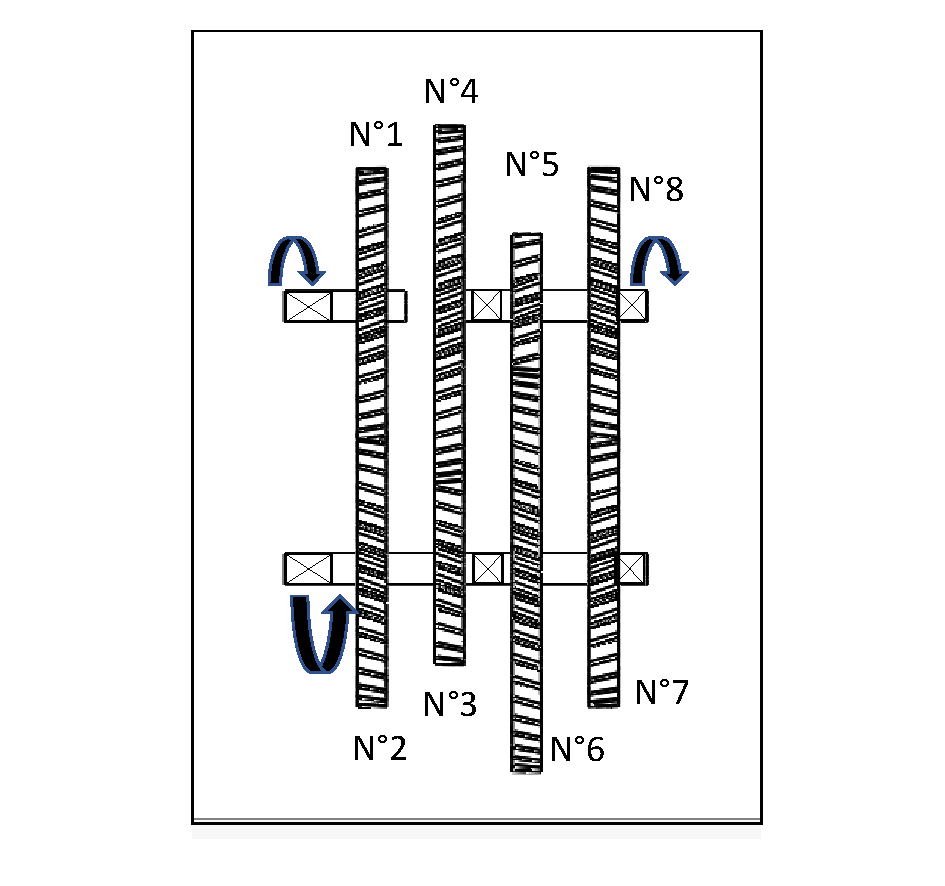
\includegraphics[width =0.5\textwidth, trim = {2cm, 0, 2cm, 0}]{Cap4_DisenoBasico/Figura/caja.pdf}
    \caption{Esquema básico del sistema de transmición}{Fuente: Elaboración propia}
    \label{fig:Transmición}
\end{figure}

\begin{table}[hbt]
    \centering
    \begin{tabular}{|c|c|}
        \hline
        \textbf{Dientes $N^{\circ}$} & \textbf{$N^{\circ}$ de dientes} \\ \hline
        1 & 34 \\ \hline
        2 & 34 \\ \hline
        3 & 51 \\ \hline
        4 & 17 \\ \hline
        5 & 45 \\ \hline
        6 & 23 \\ \hline
        7 & 34 \\ \hline
        8 & 34 \\ \hline
    \end{tabular}
    \caption{Número de dientes}
    \label{table:Transmición}
\end{table}


En la figura \ref{fig:Transmición}, se presenta un esquema de la caja de transmisión con el cual se trabajará a detalle posteriormente, esta cuenta con 8 engranajes y tres ejes, uno de entrada, uno de salida y uno intermedio. El número de dientes de cada engranaje se especifican en la tabla \ref{table:Transmición}.

\newpage